
%
%
\documentclass[11pt]{article}
\usepackage{amsmath}
\usepackage{graphicx}
\usepackage{color}
\usepackage{amsfonts}
\usepackage[T1]{fontenc}
\usepackage{libertine} \usepackage[libertine]{newtxmath}
\usepackage[margin=2.5cm,bmargin=.5cm]{geometry}
%\usepackage{showframe}
\newcommand{\cE}{\mathcal{E}}                               %
\setlength{\voffset}{-2cm}

\begin{document}

\title{Summary of summer project}

\author{Dominic Skinner}
\date{}
\maketitle
\pagenumbering{gobble}
\subsection*{Introduction}
\vspace{-6pt}
Consider a semi-infinite elastic solid with a thin strip peeled off, and the
resulting crack filled with an incompressible fluid. The motion is driven
by a bending moment applied to the ``arm'' of the solid. The aim is to be
able to write down a set of equations governing the dynamics, in particular
it is of interest to examine the relationship between the speed of traveling
wave solutions $c$, the magnitude of the bending moment $M$, and the toughness 
of the solid $K_I$. 
\\[7pt]
Relevant physical problems include both igneous intrusions beneath a volcano,
and the formation of hydrofractures in an oil
reservoir, since both involve the propagation of a crack through a brittle 
elastic solid driven by fluid injection.
\\[7pt]
This is a joint work with Tim Large, who started this project in
summer 2014.
\vspace{-4pt}
\subsection*{Set up}
\vspace{-4pt}
\begin{minipage}{0.5\linewidth}
We assume that the flow everywhere satisfies the lubrication equations. From 
fluid mechanics, we then get the equation
\vspace{-9pt}
\[12\mu c = h^2 p'\]
\vspace{-2pt}
From elasticity, using Muskhelishiveli methods, we can derive the equation
\[
\left( \begin{array}{c} p \\ 0 \end{array} \right)   =
\frac{E}{4\pi (1-\nu^2)} \int
\left(\begin{array}{cc} K_{11} & K_{12} \\ K_{21} & K_{22} \end{array} \right)
\left( \begin{array}{c} g' \\ h' \end{array} \right)  \]
\end{minipage}
\begin{minipage}{0.04\linewidth}
~
\end{minipage}
\begin{minipage}{0.5\linewidth}
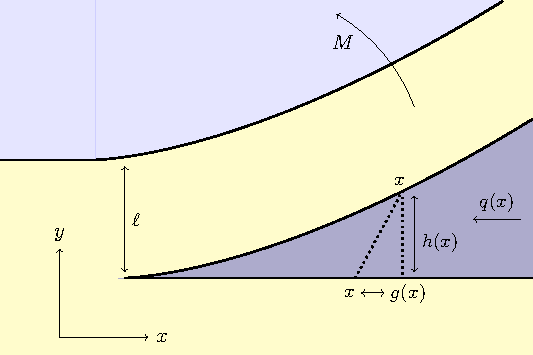
\includegraphics[scale=0.8]{Fig1.pdf}
\end{minipage}
\\[11pt]
Where $K_{ij}$ is the integral kernel specific to this geometry,
$E$ is the Young's modulus of the solid, $\nu$ is Poisson's ratio, and  $\mu$ is 
the viscosity of the fluid.
The boundary conditions on the solid at $\infty$ are governed by the bending 
moment, using the beam approximation. The boundary conditions near the crack
tip are governed by ``Linear Elastic Fracture Mechanics''. 
\\[7pt]
A problem of 
particular interest is the ``Small toughness'' problem, when 
$K_I \ll M \ell^{-3/2}$. The near tip asymptotics when $K_I=0$, namely
$h \sim x^{2/3}$ need to be reconciled with the asymptotics for 
$K_I>0$, where $h \sim x^{1/2}$. The result is a near tip boundary layer.
\\[7pt]
The equations are difficult to solve numerically as they are
a set of non-linear integro-differential equations, with multiple length scales,
and singular solutions. By approximating relevant functions as 
``known singular behaviour $\times$ piecewise linear function'', and using a
sensible spacing of grid points, the above equations can be discritized and
solved numerically.
\vspace{-4pt}
\subsection*{Results}
\vspace{-6pt}
From using analytic methods, it was found that by approaching asymptotically 
close to the crack tip, the geomety reduces to a known problem. 
This allows us to obtain the ``Small toughness'' solution
\[ c = \frac{36(1-\nu^2)^2M^3}{\pi \mu E^2 \ell^5}\left(\lambda_0 + C 
\lambda_0^{2s-1}\lambda_1 (\ell^{3/2}K_I/M)^u \right) \]
\vspace{-2pt}
The constants $\lambda_0$,$\lambda_1$, $C$, $u$,$s$, have been determined 
numerically. This result is in close agreement with numerical solutions.
%
\end{document}
